%%%%%%%%%%%%%%%%%%%%%%%%%%%%%%%%%%%%%%%%%%%%%%%%%%%%%%%%%%%%%%%%%%%%%%%%%%%%%%%%
% WeBWorK Online Homework Delivery System
% Copyright � 2000-2007 The WeBWorK Project, http://openwebwork.sf.net/
% $CVSHeader: webwork2/conf/snippets/hardcopyPreamble.tex,v 1.3 2005/09/17 20:12:01 gage Exp $
% 
% This program is free software; you can redistribute it and/or modify it under
% the terms of either: (a) the GNU General Public License as published by the
% Free Software Foundation; either version 2, or (at your option) any later
% version, or (b) the "Artistic License" which comes with this package.
% 
% This program is distributed in the hope that it will be useful, but WITHOUT
% ANY WARRANTY; without even the implied warranty of MERCHANTABILITY or FITNESS
% FOR A PARTICULAR PURPOSE.  See either the GNU General Public License or the
% Artistic License for more details.
%%%%%%%%%%%%%%%%%%%%%%%%%%%%%%%%%%%%%%%%%%%%%%%%%%%%%%%%%%%%%%%%%%%%%%%%%%%%%%%%

\batchmode
\documentclass[10pt,dvips]{amsart}
\usepackage{amsmath,amsfonts,amssymb,multicol}
\usepackage[pdftex]{graphicx}
\usepackage{epstopdf}  % allows use of eps files with pdftex
\usepackage{epsf}
\usepackage{epsfig}
\usepackage{pslatex}
\pagestyle{plain}
\textheight 9in
\oddsidemargin = -0.42in
\evensidemargin = -0.42in
\textwidth= 7.28in
\columnsep = .25in
\columnseprule = .4pt
\def\endline{\bigskip\hrule width \hsize height 0.8pt }
\newcommand{\lt}{<}
\newcommand{\gt}{>}
\newcommand{\less}{<}
\newcommand{\grt}{>}

% BEGIN capa tex macros

\newcommand{\capa}{{\sl C\kern-.10em\raise-.00ex\hbox{\rm A}\kern-.22em%
{\sl P}\kern-.14em\kern-.01em{\rm A}}}
  
\newenvironment{choicelist}
{\begin{list}{}
	{\setlength{\rightmargin}{0in}\setlength{\leftmargin}{0.13in}
	\setlength{\topsep}{0.05in}\setlength{\itemsep}{0.022in}
	\setlength{\parsep}{0in}\setlength{\belowdisplayskip}{0.04in}
	\setlength{\abovedisplayskip}{0.05in}
	\setlength{\abovedisplayshortskip}{-0.04in}
	\setlength{\belowdisplayshortskip}{0.04in}}
	}
{\end{list}}

% END capa tex macros 

\begin{document}
\voffset=-0.8in
\newpage
\setcounter{page}{1}
\begin{multicols}{2}
\columnwidth=\linewidth
%% decoded old answers, saved. (keys = 
 \end{multicols}

\noindent {\large \bf Mike Gage}
\hfill
{\large \bf {gage\_test}}
% Uncomment the line below if this course has sections. Note that this is a comment in TeX mode since this is only processed by LaTeX
%   {\large \bf { Section:  } }
\par
\noindent{\large \bf {Assignment aliasCheck  due 08/21/2012 at 12:35am EDT}}
\par\noindent \bigskip
% Uncomment and edit the line below if this course has a web page. Note that this is a comment in TeX mode.
%See the course web page for information http://yoururl/yourcourse



 \begin{multicols}{2}
\columnwidth=\linewidth
%%%%%%%%%%%%%%%%%%%%%%%%%%%%%%%%%%%%%%%%%%%%%%%%%%%%%%%%%%%%%%%%%%%%%%%%%%%%%%%%
% WeBWorK Online Homework Delivery System
% Copyright � 2000-2007 The WeBWorK Project, http://openwebwork.sf.net/
% $CVSHeader: webwork2/conf/snippets/hardcopyProblemDivider.tex,v 1.3 2004/06/24 21:10:50 dpvc Exp $
% 
% This program is free software; you can redistribute it and/or modify it under
% the terms of either: (a) the GNU General Public License as published by the
% Free Software Foundation; either version 2, or (at your option) any later
% version, or (b) the "Artistic License" which comes with this package.
% 
% This program is distributed in the hope that it will be useful, but WITHOUT
% ANY WARRANTY; without even the implied warranty of MERCHANTABILITY or FITNESS
% FOR A PARTICULAR PURPOSE.  See either the GNU General Public License or the
% Artistic License for more details.
%%%%%%%%%%%%%%%%%%%%%%%%%%%%%%%%%%%%%%%%%%%%%%%%%%%%%%%%%%%%%%%%%%%%%%%%%%%%%%%%

\medskip
\goodbreak
\hrule
\nobreak
\smallskip
%% decoded old answers, saved. (keys = 
{\bf 1. {\footnotesize (1 pt) local\-/setaliasCheck\-/htmlAliasCheck\-/htmlAliasCheck.pg}}\newline {\bf  Check that the alias command works to find HTML files } \par 
All of these tests should succeed.
\par 

This should find a static .gif graph file in the same directory.\par 
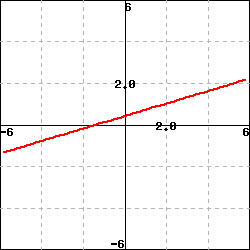
\includegraphics[width=0.8\linewidth]{/Volumes/WW_test/opt/webwork/courses/gage_test/html/tmp/images/14d95a9e-f484-3f4b-9c07-55615f08780f___76db5f5a-d18a-301e-be67-af9269dc1a5b.png}
\par 
\-/Volumes\-/WW\_test\-/opt\-/webwork\-/courses\-/gage\_test\-/html\-/tmp\-/images\-/14d95a9e-f484-3f4b-9c07-55615f08780f\_\_\_76db5f5a-d18a-301e-be67-af9269dc1a5b.png \par 
This should find an html file in the same directory.
{\bf \underline{url }} should bring up a new html page.
\par 
\-/Volumes\-/WW\_test\-/opt\-/webwork\-/courses\-/gage\_test\-/html\-/tmp\-/images\-/14d95a9e-f484-3f4b-9c07-55615f08780f\_\_\_76db5f5a-d18a-301e-be67-af9269dc1a5b.png
\par 

  prettyprint resources: \leavevmode\\\relax {\tiny\begin{tabular}{| c | c |}\hline
\multicolumn{2}{|c|}{HASH(0x10a0370a8)}\\ \hline
prob14 & \begin{tabular}{| c | c |}\hline
\multicolumn{2}{|c|}{PGresource=HASH(0x10a1d0a20)}\\ \hline
DEBUG\_messages & (  )\\ \hline
WARNING\_messages & (  )\\ \hline
cache\_info & \begin{tabular}{| c | c |}\hline
\multicolumn{2}{|c|}{HASH(0x10a1d09c0)}\\ \hline
\end{tabular}
\\ \hline
convert & \begin{tabular}{| c | c |}\hline
\multicolumn{2}{|c|}{HASH(0x10a1d08a0)}\\ \hline
from\_path & /Volumes/WW\_test/opt/webwork/courses/gage\_test/templates/local/setaliasCheck/htmlAliasCheck/prob14.gif\\ \hline
from\_type & gif\\ \hline
needed & 1\\ \hline
to\_path & /Volumes/WW\_test/opt/webwork/courses/gage\_test/html/tmp/images/14d95a9e-f484-3f4b-9c07-55615f08780f\_\_\_76db5f5a-d18a-301e-be67-af9269dc1a5b.png\\ \hline
to\_type & png\\ \hline
\end{tabular}
\\ \hline
copy\_link & \begin{tabular}{| c | c |}\hline
\multicolumn{2}{|c|}{HASH(0x10a1d0948)}\\ \hline
copy\_to\_path & \\ \hline
link\_to\_path & \\ \hline
type & \\ \hline
\end{tabular}
\\ \hline
id & prob14\\ \hline
parent\_alias & PGalias has too much info. Try $PG->{PG_alias}->{resource_list}\\ \hline
parent\_file\_id & local/setaliasCheck/htmlAliasCheck/htmlAliasCheck.pg\\ \hline
path & \begin{tabular}{| c | c |}\hline
\multicolumn{2}{|c|}{HASH(0x10a1d0720)}\\ \hline
content & /Volumes/WW\_test/opt/webwork/courses/gage\_test/templates/local/setaliasCheck/htmlAliasCheck/prob14.gif\\ \hline
is\_accessible & 0\\ \hline
is\_complete & 1\\ \hline
\end{tabular}
\\ \hline
recorded\_uri & \\ \hline
return\_uri & \\ \hline
type & gif\\ \hline
unique\_id & 14d95a9e-f484-3f4b-9c07-55615f08780f\_\_\_76db5f5a-d18a-301e-be67-af9269dc1a5b\\ \hline
uri & \begin{tabular}{| c | c |}\hline
\multicolumn{2}{|c|}{HASH(0x10a1d0828)}\\ \hline
content & /Volumes/WW\_test/opt/webwork/courses/gage\_test/html/tmp/images/14d95a9e-f484-3f4b-9c07-55615f08780f\_\_\_76db5f5a-d18a-301e-be67-af9269dc1a5b.png\\ \hline
is\_accessible & 1\\ \hline
is\_complete & 1\\ \hline
\end{tabular}
\\ \hline
\end{tabular}
\\ \hline
\end{tabular}
}%%%%%%%%%%%%%%%%%%%%%%%%%%%%%%%%%%%%%%%%%%%%%%%%%%%%%%%%%%%%%%%%%%%%%%%%%%%%%%%%
% WeBWorK Online Homework Delivery System
% Copyright � 2000-2007 The WeBWorK Project, http://openwebwork.sf.net/
% $CVSHeader: webwork2/conf/snippets/hardcopyProblemDivider.tex,v 1.3 2004/06/24 21:10:50 dpvc Exp $
% 
% This program is free software; you can redistribute it and/or modify it under
% the terms of either: (a) the GNU General Public License as published by the
% Free Software Foundation; either version 2, or (at your option) any later
% version, or (b) the "Artistic License" which comes with this package.
% 
% This program is distributed in the hope that it will be useful, but WITHOUT
% ANY WARRANTY; without even the implied warranty of MERCHANTABILITY or FITNESS
% FOR A PARTICULAR PURPOSE.  See either the GNU General Public License or the
% Artistic License for more details.
%%%%%%%%%%%%%%%%%%%%%%%%%%%%%%%%%%%%%%%%%%%%%%%%%%%%%%%%%%%%%%%%%%%%%%%%%%%%%%%%

\medskip
\goodbreak
\hrule
\nobreak
\smallskip
%% decoded old answers, saved. (keys = 
%%%%%%%%%%%%%%%%%%%%%%%%%%%%%%%%%%%%%%%%%%%%%%%%%%%%%%%%%%%%%%%%%%%%%%%%%%%%%%%%
% WeBWorK Online Homework Delivery System
% Copyright � 2000-2007 The WeBWorK Project, http://openwebwork.sf.net/
% $CVSHeader: webwork2/conf/snippets/hardcopyProblemDivider.tex,v 1.3 2004/06/24 21:10:50 dpvc Exp $
% 
% This program is free software; you can redistribute it and/or modify it under
% the terms of either: (a) the GNU General Public License as published by the
% Free Software Foundation; either version 2, or (at your option) any later
% version, or (b) the "Artistic License" which comes with this package.
% 
% This program is distributed in the hope that it will be useful, but WITHOUT
% ANY WARRANTY; without even the implied warranty of MERCHANTABILITY or FITNESS
% FOR A PARTICULAR PURPOSE.  See either the GNU General Public License or the
% Artistic License for more details.
%%%%%%%%%%%%%%%%%%%%%%%%%%%%%%%%%%%%%%%%%%%%%%%%%%%%%%%%%%%%%%%%%%%%%%%%%%%%%%%%

\medskip
\goodbreak
\hrule
\nobreak
\smallskip
%% decoded old answers, saved. (keys = 
%%%%%%%%%%%%%%%%%%%%%%%%%%%%%%%%%%%%%%%%%%%%%%%%%%%%%%%%%%%%%%%%%%%%%%%%%%%%%%%%
% WeBWorK Online Homework Delivery System
% Copyright � 2000-2007 The WeBWorK Project, http://openwebwork.sf.net/
% $CVSHeader: webwork2/conf/snippets/hardcopyProblemDivider.tex,v 1.3 2004/06/24 21:10:50 dpvc Exp $
% 
% This program is free software; you can redistribute it and/or modify it under
% the terms of either: (a) the GNU General Public License as published by the
% Free Software Foundation; either version 2, or (at your option) any later
% version, or (b) the "Artistic License" which comes with this package.
% 
% This program is distributed in the hope that it will be useful, but WITHOUT
% ANY WARRANTY; without even the implied warranty of MERCHANTABILITY or FITNESS
% FOR A PARTICULAR PURPOSE.  See either the GNU General Public License or the
% Artistic License for more details.
%%%%%%%%%%%%%%%%%%%%%%%%%%%%%%%%%%%%%%%%%%%%%%%%%%%%%%%%%%%%%%%%%%%%%%%%%%%%%%%%

\medskip
\goodbreak
\hrule
\nobreak
\smallskip
%% decoded old answers, saved. (keys = 
%% decoded old answers, saved. (keys = 
 \end{multicols}


\noindent {\tiny Generated by \copyright WeBWorK, http://webwork.maa.org, Mathematical Association of America}

 \begin{multicols}{2}
\columnwidth=\linewidth


%%%%%%%%%%%%%%%%%%%%%%%%%%%%%%%%%%%%%%%%%%%%%%%%%%%%%%%%%%%%%%%%%%%%%%%%%%%%%%%%
% WeBWorK Online Homework Delivery System
% Copyright � 2000-2007 The WeBWorK Project, http://openwebwork.sf.net/
% $CVSHeader: webwork2/conf/snippets/hardcopyPostamble.tex,v 1.2 2003/12/09 01:12:29 sh002i Exp $
% 
% This program is free software; you can redistribute it and/or modify it under
% the terms of either: (a) the GNU General Public License as published by the
% Free Software Foundation; either version 2, or (at your option) any later
% version, or (b) the "Artistic License" which comes with this package.
% 
% This program is distributed in the hope that it will be useful, but WITHOUT
% ANY WARRANTY; without even the implied warranty of MERCHANTABILITY or FITNESS
% FOR A PARTICULAR PURPOSE.  See either the GNU General Public License or the
% Artistic License for more details.
%%%%%%%%%%%%%%%%%%%%%%%%%%%%%%%%%%%%%%%%%%%%%%%%%%%%%%%%%%%%%%%%%%%%%%%%%%%%%%%%

\end{multicols}
\vfill
\end{document}
